\documentclass{article}
\usepackage[T1]{fontenc}
\usepackage[utf8]{inputenc}

\makeatletter \providecommand{\tabularnewline}{\\}

\usepackage{cec2003,multicol,times}
\usepackage{graphicx}
\usepackage{hyphenat}
\usepackage{hyperref}
\usepackage{indentfirst}
\usepackage[english]{babel}
\makeatother

\begin{document}

\pagestyle{empty} 
\sloppy
\twocolumn[
\title{Análise do Espectro Raman de amostras de cachaça através de PCA e Redes Neurais Artificiais\\\vspace{0.5cm}}
\begin{center}
\textbf{Daniel S. Costa} \\
UTFPR\\
Av. Sete de Setembro, 3165 \\
80230-901 Curitiba, Brazil \\\vspace{0.5cm}
\end{center}
]

\begin{abstract}
O presente trabalho valida a utilização de redes neurais artificiais na interpretação de dados do espectro Raman de amostras de cachaça. Combinando a modelagem a técnica PCA(Principal Component Analysis) de forma a maximizar a taxa de sucesso obtida. \vspace{2cm}
\end{abstract}

\section{Introdução}
\vspace{1cm} 
Este trabalho baseia-se no artigo [1] em que o espectro Raman de amostras de cachaças são submetidas a técnica PCA(Principal Component Analysis) de forma a separar as principais componentes da assinatura Raman tornando possível a visualização clusterizada de amostras contaminados por metanol ou não.

De forma complementar ao artigo citado, uma rede neural artificial foi treinada buscando obter a mesma classificação obtida pela técnica do PCA. Contudo, o número de amostras para o treinamento da rede é pequeno, sobretudo quando leva-se em consideração a quantidade de features que são 1024. Assim, observou-se que a rede neural não obteve a assertividade esperada, mesmo testando diferentes quantidade de neurônios na camada escondida da rede.

Outra abordagem adotada foi submeter as amostras ao PCA, e submeter os valores resultantes das 2 principais componentes a rede neural. Deste modo, o teste obteve uma taxa de sucesso de 80\%.

Os arquivos das amostras, bem como o código fonte da aplicação e relatórios elaborados estão disponíveis através do : \href{https://github.com/danielscosta/mestrado/tree/master/disciplinas/Inteligencia_Artificial/projeto}{link}.

Através dos experimentos realizados pode-se concluir que para uma grande quantidade de features e poucas amostras, a rede neural utilizada é ineficaz na classificação dos dados. Uma vez obtida as principais componentes da amostra através do PCA, a classificação se torna possível por conta da diminuição da quantidade de features avaliadas.

\vspace{2cm}
\subsection{Descrição do Problema}
\vspace{1cm} A Espectroscopia Raman é um técnica capaz de revelar importantes informações sobre a composição de um material analisado. Podendo, até mesmo, ser utilizado na classificação biológica, uma vez que, células de diferentes organismos apresentam diferentes composições químicas.
Contudo a interpretação da assinatura gerado pela medição do espectro Raman pode ser uma tarefa desafiadora, uma vez que determinar quais os picos da curva são relevantes na distinção de uma material de outro requer treinamento e experiência por parte de quem analisa tal assinatura.

\subsection{Motivação}
\vspace{1cm} Criar metodologias e automatizações na análise do dados da espectroscopia Raman pode vir a facilitar o processo de identificação e classificação de materias ou seres vivos. O que se mostra relevantes na busca de contaminantes em um produto ou até mesmo na identificação de uma bactéria/fungo num processo infeccioso.

\vspace{2cm}
\section{Revisão da Literatura}
\subsection{Descrição da técnica utilizada}
As redes neurais artificiais possuem vastas arquiteturas. As disposições de suas camadas e como os neurônios se ligam vão determinar para qual tipo de problema aquela configuração melhor se aplica. Neste trabalho, optou-se por utilizar multilayer perceptron com o propósito de classificar amostras com teor de Metanol superior a 10\%.\vspace{4cm}

Outra técnica utilizada para este trabalho foi o PCA - Principal Component Analysis. Que realiza um transformada matemática através da features das amostras de forma a criar um novo espaço amostral em que a significância de cada feature é mensurada. Feito isto, optou-se por trabalhar com as 2 componentes de maior significância (96\% e 2\%) como inputs uma rede neural multilayer perceptron.

Para ambas técnicas descritas foram implementados códigos na linguagem python, utilzando-se da biblioteca sklearn.

\subsection{Descrição das abordagens relacionadas}
\vspace{1cm} O artigo[1] que dá base a este trabalho apresenta de forma detalhada a aplicabilidade da espectroscopia Raman na identificação de materiais. E utiliza-se do PCA para clusterizar as amostras de forma a evidenciar o grupo de características a ser analisado.

A matéria de estudo do referido artigo[1] é a cachaça, uma bebida, composta sobretudo por água, etanol e metanol. Para consumo humano, tal bebida não deve conter quantidades significativas de metanol, pois este composto é danoso a saúde humana, podendo em níveis elevados levar até mesmo a morte.

Foram montados dois conjuntos de amostras, um com uma mistura de água, etanol e metanol, e o outro com cachaças adquiridas em mercados. Para ambos os conjuntos de amostras, os espectros Raman foram mensurados em laboratório gerando arquivos que contém a representação matemática da curva de intensidade luminosa do espectro Raman. O primeiro grupo simulou a composição da cachaça e foi usado como base para definir a transformação de espaço realizada no PCA. No segundo grupo, de modo aleatório, algumas cachaças tiveram metanol misturado a sua composição, de forma a simular uma contaminação.

Nos experimentos realizados, foi avaliado se através do PCA seria possível distinguir das amostras do primeiro conjunto as que continham um teor de metanol. E o resultado mostrou uma separação linear dos que continham uma quantidade significativa de metanol das que não continham. Posteriormente, o segundo conjunto de amostras foi submetido ao PCA, utilizando-se da base de coeficientes obtida pelo primeiro conjunto de forma a revelar se com a mesma metologia, seria possível identificar contaminação em produtos de mercado. E o resultado foi positivo.

Como trabalho futuro o artigo[1] sugere a associação de uma rede neural artificial para avaliar a contaminação por metanol. Uma vez que esta técnica poderia oferecer uma automatização a esta análise. Por isto, este trabalho propoe-se esta atividade.

\vspace{2cm}
\section{Metodologia}
\vspace{1cm} O autor do artigo[1] referenciado forneceu os arquivos contendo a representação matemática da curva de intensidade luminosa do espectro Raman para os dois grupos amostrais citados anteriormente.

Os dados obtidos foram normalizados e o primeiro grupo de dados foi utilizado como base de treinamento da rede neural, e o segundo como base de testes. Foram comparadas duas abordagem, a primeira os dados foram submetidos diretamente a rede neural, com todas as suas features e na segunda, os dados passaram pelo PCA, e apenas as duas principais componentes foram submetidas a rede neural.

A comparação proposta visa avaliar se a rede neural artificial multilayer perceptron poderia promover a mesma transformação de espaço que ocorre no PCA e classificar o resultados de forma assertiva.

\vspace{2cm}
\section{Simulações e Resultados}
\vspace{1cm} É interessante que a abordagem possa ser simulada e
os resultados sejam apresentados nesta seção. Neste caso, o modelo
simulado baseado em uma técnica de IA deve ser avaliado e, se for o caso,
comparado com outro modelo, para verificar se há vantagem no uso
da técnica. \vspace{2cm}

\begin{figure}[ht]
\centering
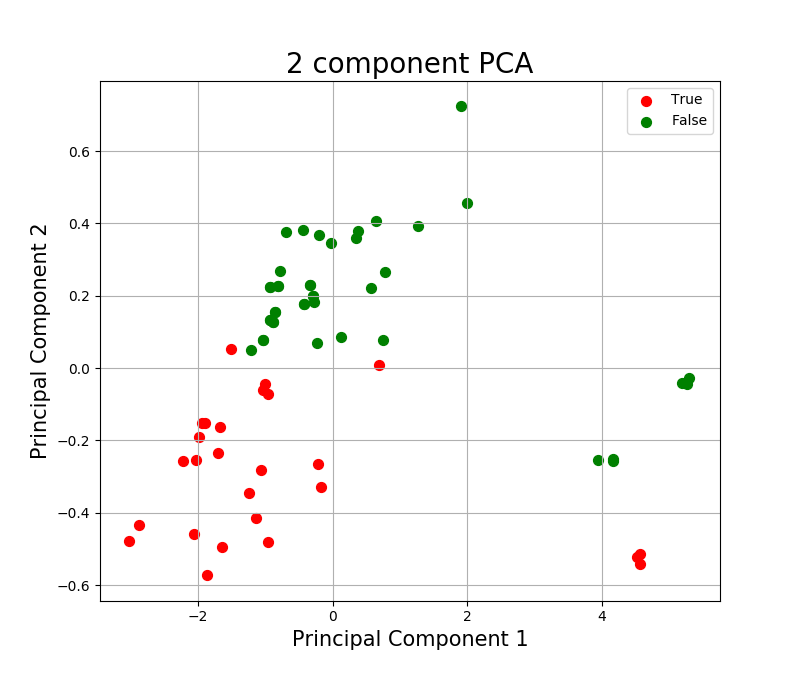
\includegraphics[width=8.5cm]{pca}
\caption{Plot das Principais Componentes do espectro Raman após normalização dos dados. PC1: 96\% significância, PC2: 2\% de significância. True = Amostra Acima de 10\% Metanol, False = Amostra Abaixo de 10\% Metanol}
\label{pca}
\end{figure}

\begin{figure}[ht]
\centering
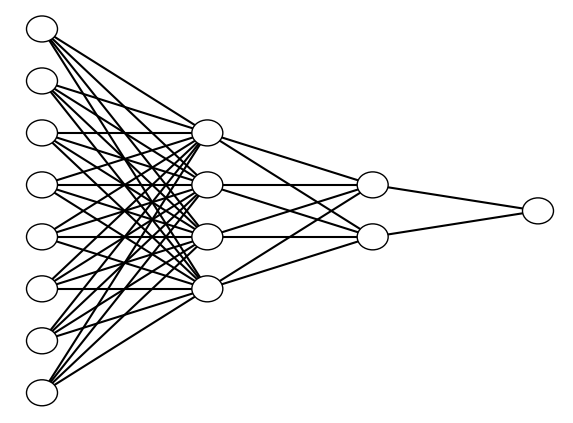
\includegraphics[width=8.5cm]{rna_4_2}
\caption{Representação da Rede Neural 1024 inputs(foram desenhados apenas 8 inputs para facilitar visualização), com 2 camadas escondidas de 4 e 2 neurônios, respectivamente.}
\label{rna_4_2}
\end{figure}

\begin{figure}[ht]
\centering
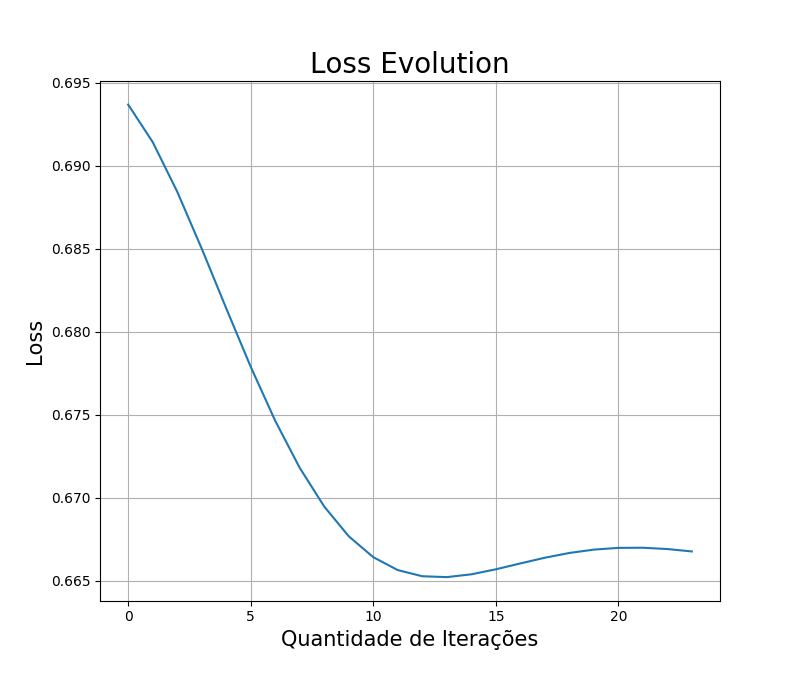
\includegraphics[width=8.5cm]{rna_4_2_loss}
\caption{Decréscimo do erro a cada iteração da rede neural artificial para a configuração com 2 camadas escondidas de 4 e 2 neurônios, respectivamente}
\label{rna_4_2_loss}
\end{figure}

\begin{figure}[ht]
\centering
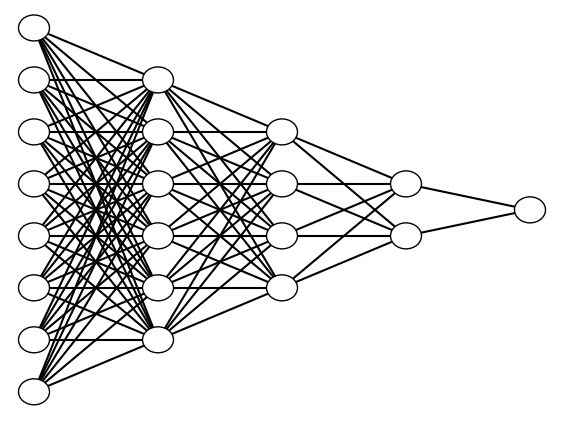
\includegraphics[width=8.5cm]{rna_6_4_2}
\caption{Representação da Rede Neural 1024 inputs(foram desenhados apenas 8 inputs para facilitar visualização), com 3 camadas escondidas de 6, 4 e 2 neurônios, respectivamente.}
\label{rna_6_4_2}
\end{figure}

\begin{figure}[ht]
\centering
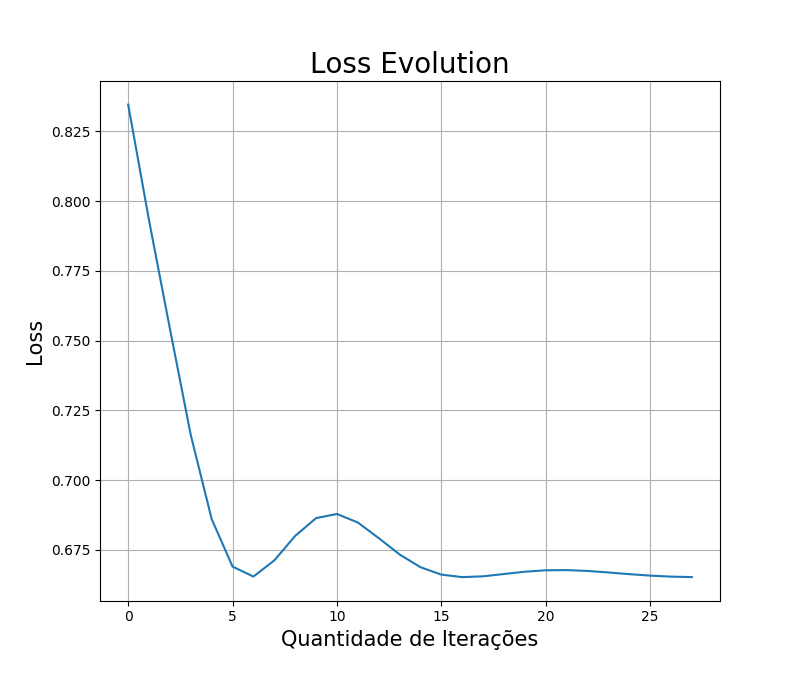
\includegraphics[width=8.5cm]{rna_6_4_2_loss}
\caption{Decréscimo do erro a cada iteração da rede neural artificial para a configuração com 3 camadas escondidas de 6, 4 e 2 neurônios, respectivamente}
\label{rna_6_4_2_loss}
\end{figure}

\begin{figure}[ht]
\centering
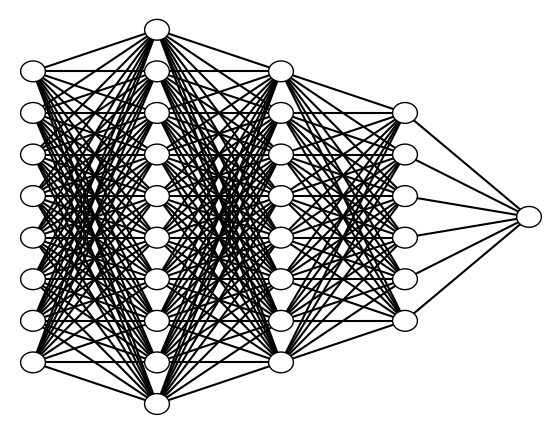
\includegraphics[width=8.5cm]{rna_10_8_6}
\caption{Representação da Rede Neural 1024 inputs(foram desenhados apenas 8 inputs para facilitar visualização), com 3 camadas escondidas de 10, 8 e 6 neurônios, respectivamente.}
\label{rna_10_8_6}
\end{figure}

\begin{figure}[ht]
\centering
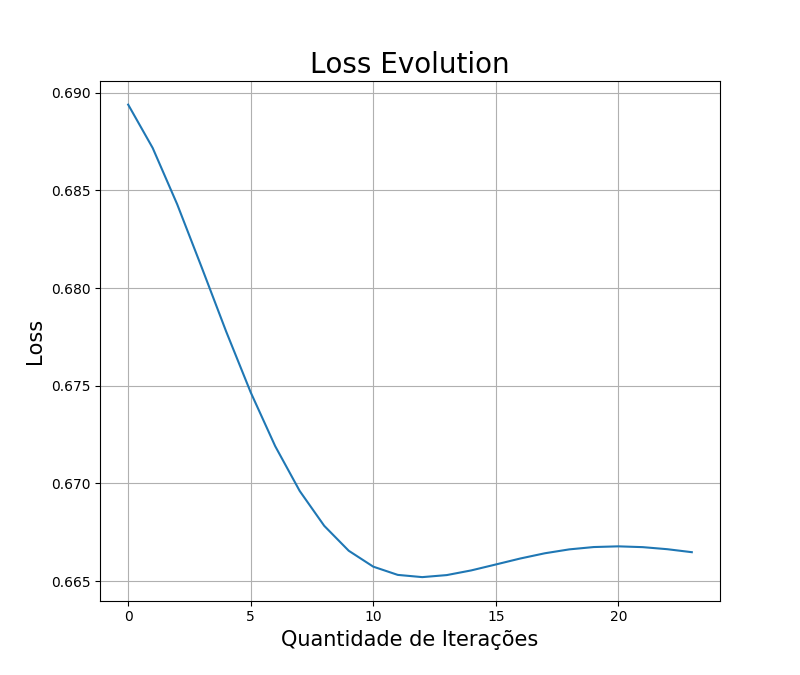
\includegraphics[width=8.5cm]{rna_10_8_6_loss}
\caption{Decréscimo do erro a cada iteração da rede neural artificial para a configuração com 3 camadas escondidas de 6, 4 e 2 neurônios, respectivamente}
\label{rna_10_8_6_loss}
\end{figure}

\begin{figure}[ht]
\centering
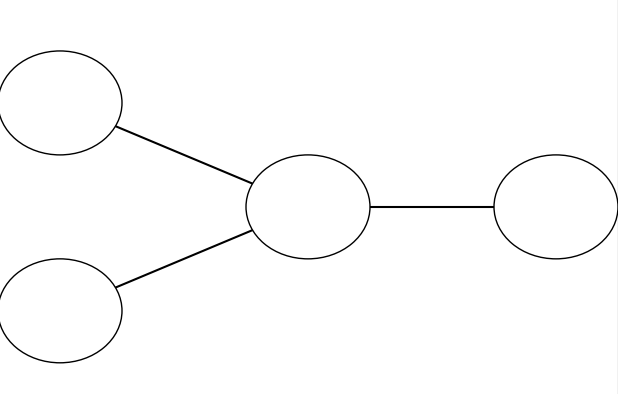
\includegraphics[width=8.5cm]{rna_pca_1}
\caption{Representação da Rede Neural após PCA, 2 inputs com 1 camada escondida de 1 neurônio}
\label{rna_pca_1}
\end{figure}

\begin{figure}[ht]
\centering
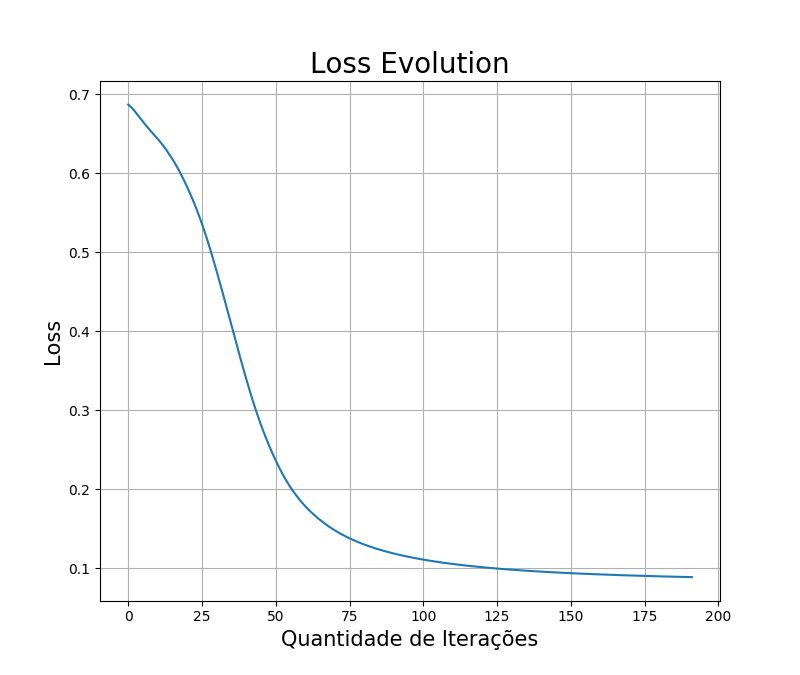
\includegraphics[width=8.5cm]{rna_pca_1_loss}
\caption{Decréscimo do erro a cada iteração da rede neural artificial para a configuração com 1 camada escondida de 1 neurônio}
\label{rna_pca_1_loss}
\end{figure}

\section{Conclusões}
\vspace{1cm} Esta seção deverá trazer as conclusões a respeito da
abordagem e resultados obtidos. \vspace{2cm}

\section*{Referências}
\vspace{1cm} [1] R. E. De Góes, L. V. M. Fabris, M. Muller, and J. L. Fabris, “Light-
assisted detection of methanol in contaminated spirits,” Journal of
Lightwave Technology, vol. 34, no. 19, pp. 4499–4505, 2016.

\end{document}